\documentclass[../lab2.tex]{subfiles}

\begin{document}
    
    \begin{figure}[!htb]
        \begin{minipage}{0.48\textwidth}
            \centering
            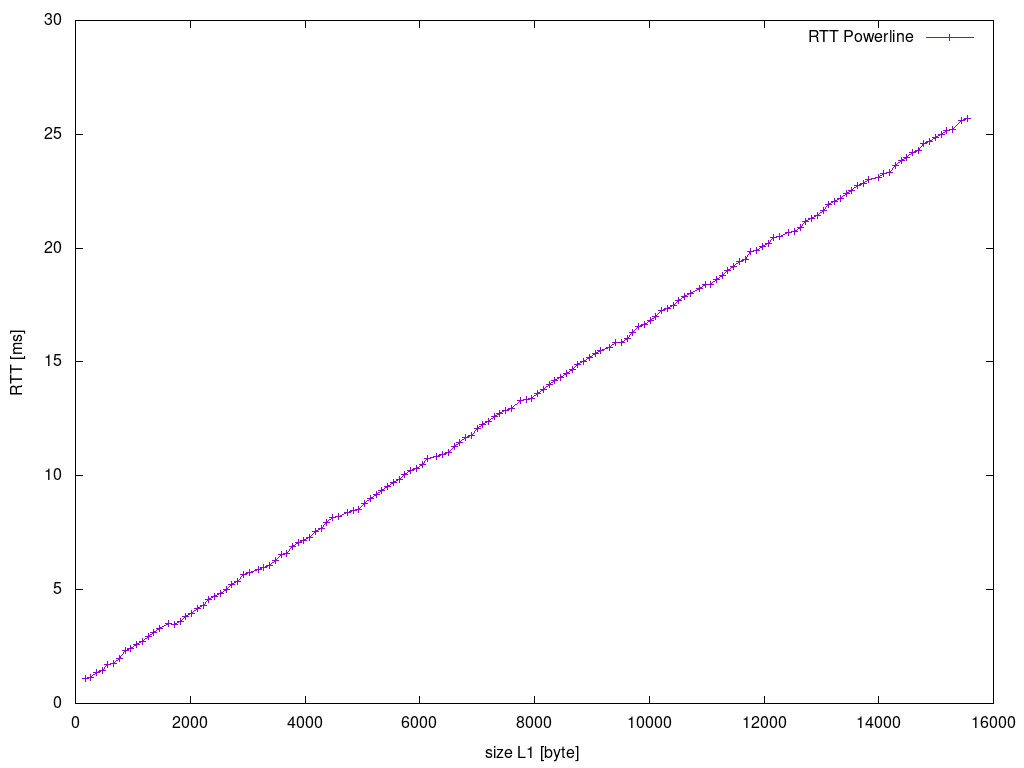
\includegraphics[width=1\linewidth]{RTTP.png}
            \vspace{-20pt}
            \caption{VTx}\label{RTTP}
        \end{minipage}\hfill
        \begin{minipage}{0.48\textwidth}
            \centering
            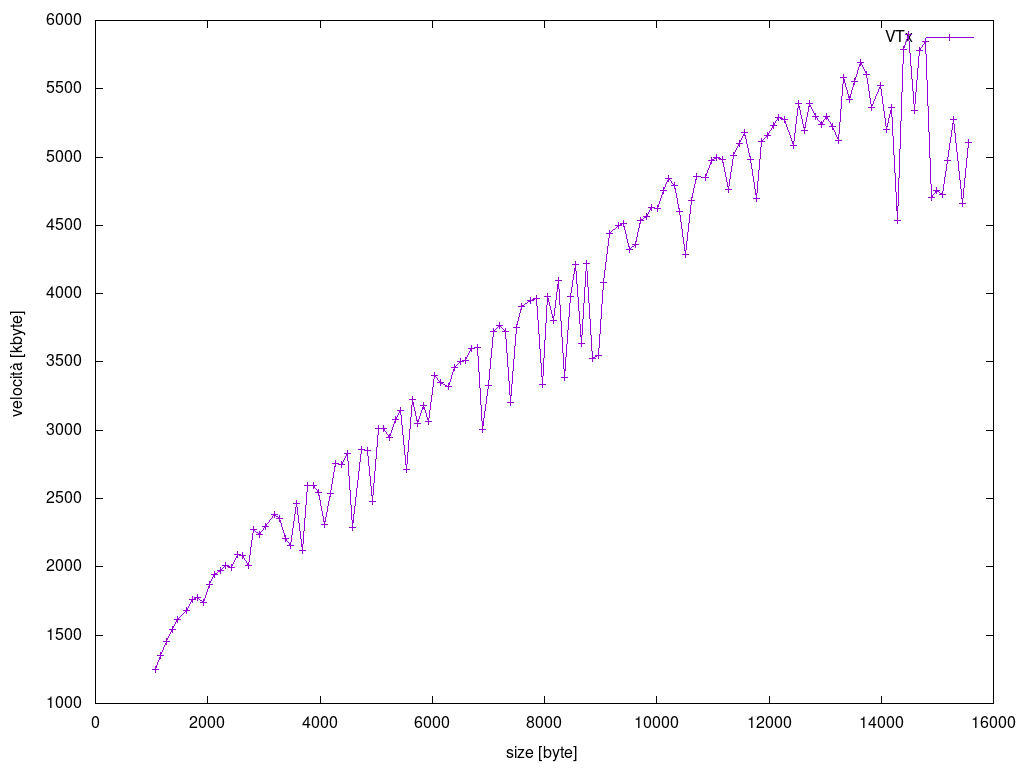
\includegraphics[width=1\linewidth]{VTxP.png}
            \vspace{-20pt}
            \caption{VTx}\label{VTxP}
        \end{minipage}
    \end{figure}

    Abbiamo ricavato questo modello per approssimare questo scenario ipotizzando 
    tre velocita' diverse all'interno del modello, ma una incognita

    \begin{equation}
        \centering
        \begin{cases}
            RTT = \frac{2D}{V_{TX1}} +\frac{4D}{V_{TX2}} +\frac{6D}{V_{TX3}} + T_\eta  \qquad \, \, \, D < 1500 \\
            \\
            RTT = \frac{2D}{V_{TX1}} +\frac{4MTU}{V_{TX2}} +\frac{6D}{V_{TX3}} + T_\eta  \qquad D > 1500
        \end{cases}
    \end{equation}

    Dove:

    \begin{itemize}
        \item $V_{TX1}$ e' la velocita' tra Pc Live Linux e il primo adattatore powerline \\
        \item $V_{TX2}$ e' la velocita' incognita tra gli adattatori powerline \\ 
        \item $V_{TX3}$ e' 100 Mb/s
    \end{itemize}

    Dal grafico si puo' notare un comportamento oscillante e poco stabile probabilmente
    dovuto a rumore e congestione all'interno della rete elettrica.

\end{document}